\documentclass[11pt, titlepage]{article}
\usepackage{amsmath,amsthm,amssymb}
\usepackage{hyperref, pgf, tikz}
\usepackage{fancyhdr}
\usetikzlibrary{arrows}
\usepackage[margin=1.25in]{geometry}
\usepackage{graphicx}                     
\pagestyle{fancy}
\usepackage{array}
%\usepackage{wrapfig}

\lhead{Lab \#4}
\rhead{\thepage}
\cfoot{}

\title{Torques, Equilibrium, and Center of Gravity\\ \ \\ \large Lab \#4}
\author{Name: Avery Karlin \\ Partner: Nicholas Yang}
\date{}
\begin{document}

\maketitle

\begin{center}
\LARGE Torques, Equilibrium, and Center of Gravity
\end{center}

\section*{Objective}
The objective of the lab is to create mechanical equilibrium, and determine moment arms, masses, and torque by creating mechanical equilibrium, both by measurement and calculation.
\section*{Introduction}

Static equilibrium is the idea of being fully stationary, such that net torque and net force equal 0, when velocity and rotational velocity are both 0. The former condition is that of translational equilibrium, such that there is no translational acceleration, while the latter is that of rotational equlibrium, such that there is no rotational acceleration. The torque is the result of force being applied at some moment arm, or distance from the axis of rotation, such that $\tau = \vec{F}\vec{r}$, where positive is the convention for counterclockwise torque, and clockwise torque is negative.

The center of gravity of a body is the point such that torques due to gravity about an axis through that point is 0. The center of mass, on the other hand, is the point such that translational motion is through that point. When the mass of a body is concentrated with even density around the center of mass, the center of mass is also the center of gravity.

Uniform linear density allows the mass of lengths of the meter stick to be known, such that if mass is uniformly dispersed, there is some value, $\mu = \frac{m/L}$, such that mass can be found by multiplying the overall linear density by the length.

\section*{Procedures and Results}

First, we must set up the meter stick such that it can rotate about an axis, created by a clamp, but such that it is fixed in place, at translational equilibrium. After that, we are able to fix masses to sliding clamps on the meter stick itself, such that we can test the movement and mass of the bodies, to find static equilibrium.

For the first three (and the fourth case, instructors choice, which we don't do), we place the axis of rotation at the center of gravity, so that we can assume that torque due to gravity is 0, focusing purely on the masses. For case 1, we know the mass of two masses, and the location of one, testing different locations to determine the point where net torque equals 0. For case 2, we have three masses which we know, two locations which we know, and determine the third by the same means. For case 3, we know the location of one, but not the mass, and the mass of the other, but not the location, and we test different locations to reach equilibrium, which allows the original mass to be calculated.

For the final two cases, the meter stick does not rotate about the center of gravity, such that we move it to some other point, where we can't discount gravitational force on the different parts of the meter stick. In the 5th case, we placed a mass on the end, determining the support point of static equilibrium, accounting for gravitational torque. Next, we placed the same mass on that one end, but added a mass to the other end at different locations, determining the support position of static equlibrium each time.

\begin{figure}[p]
\centering
\hspace*{-10.5cm}
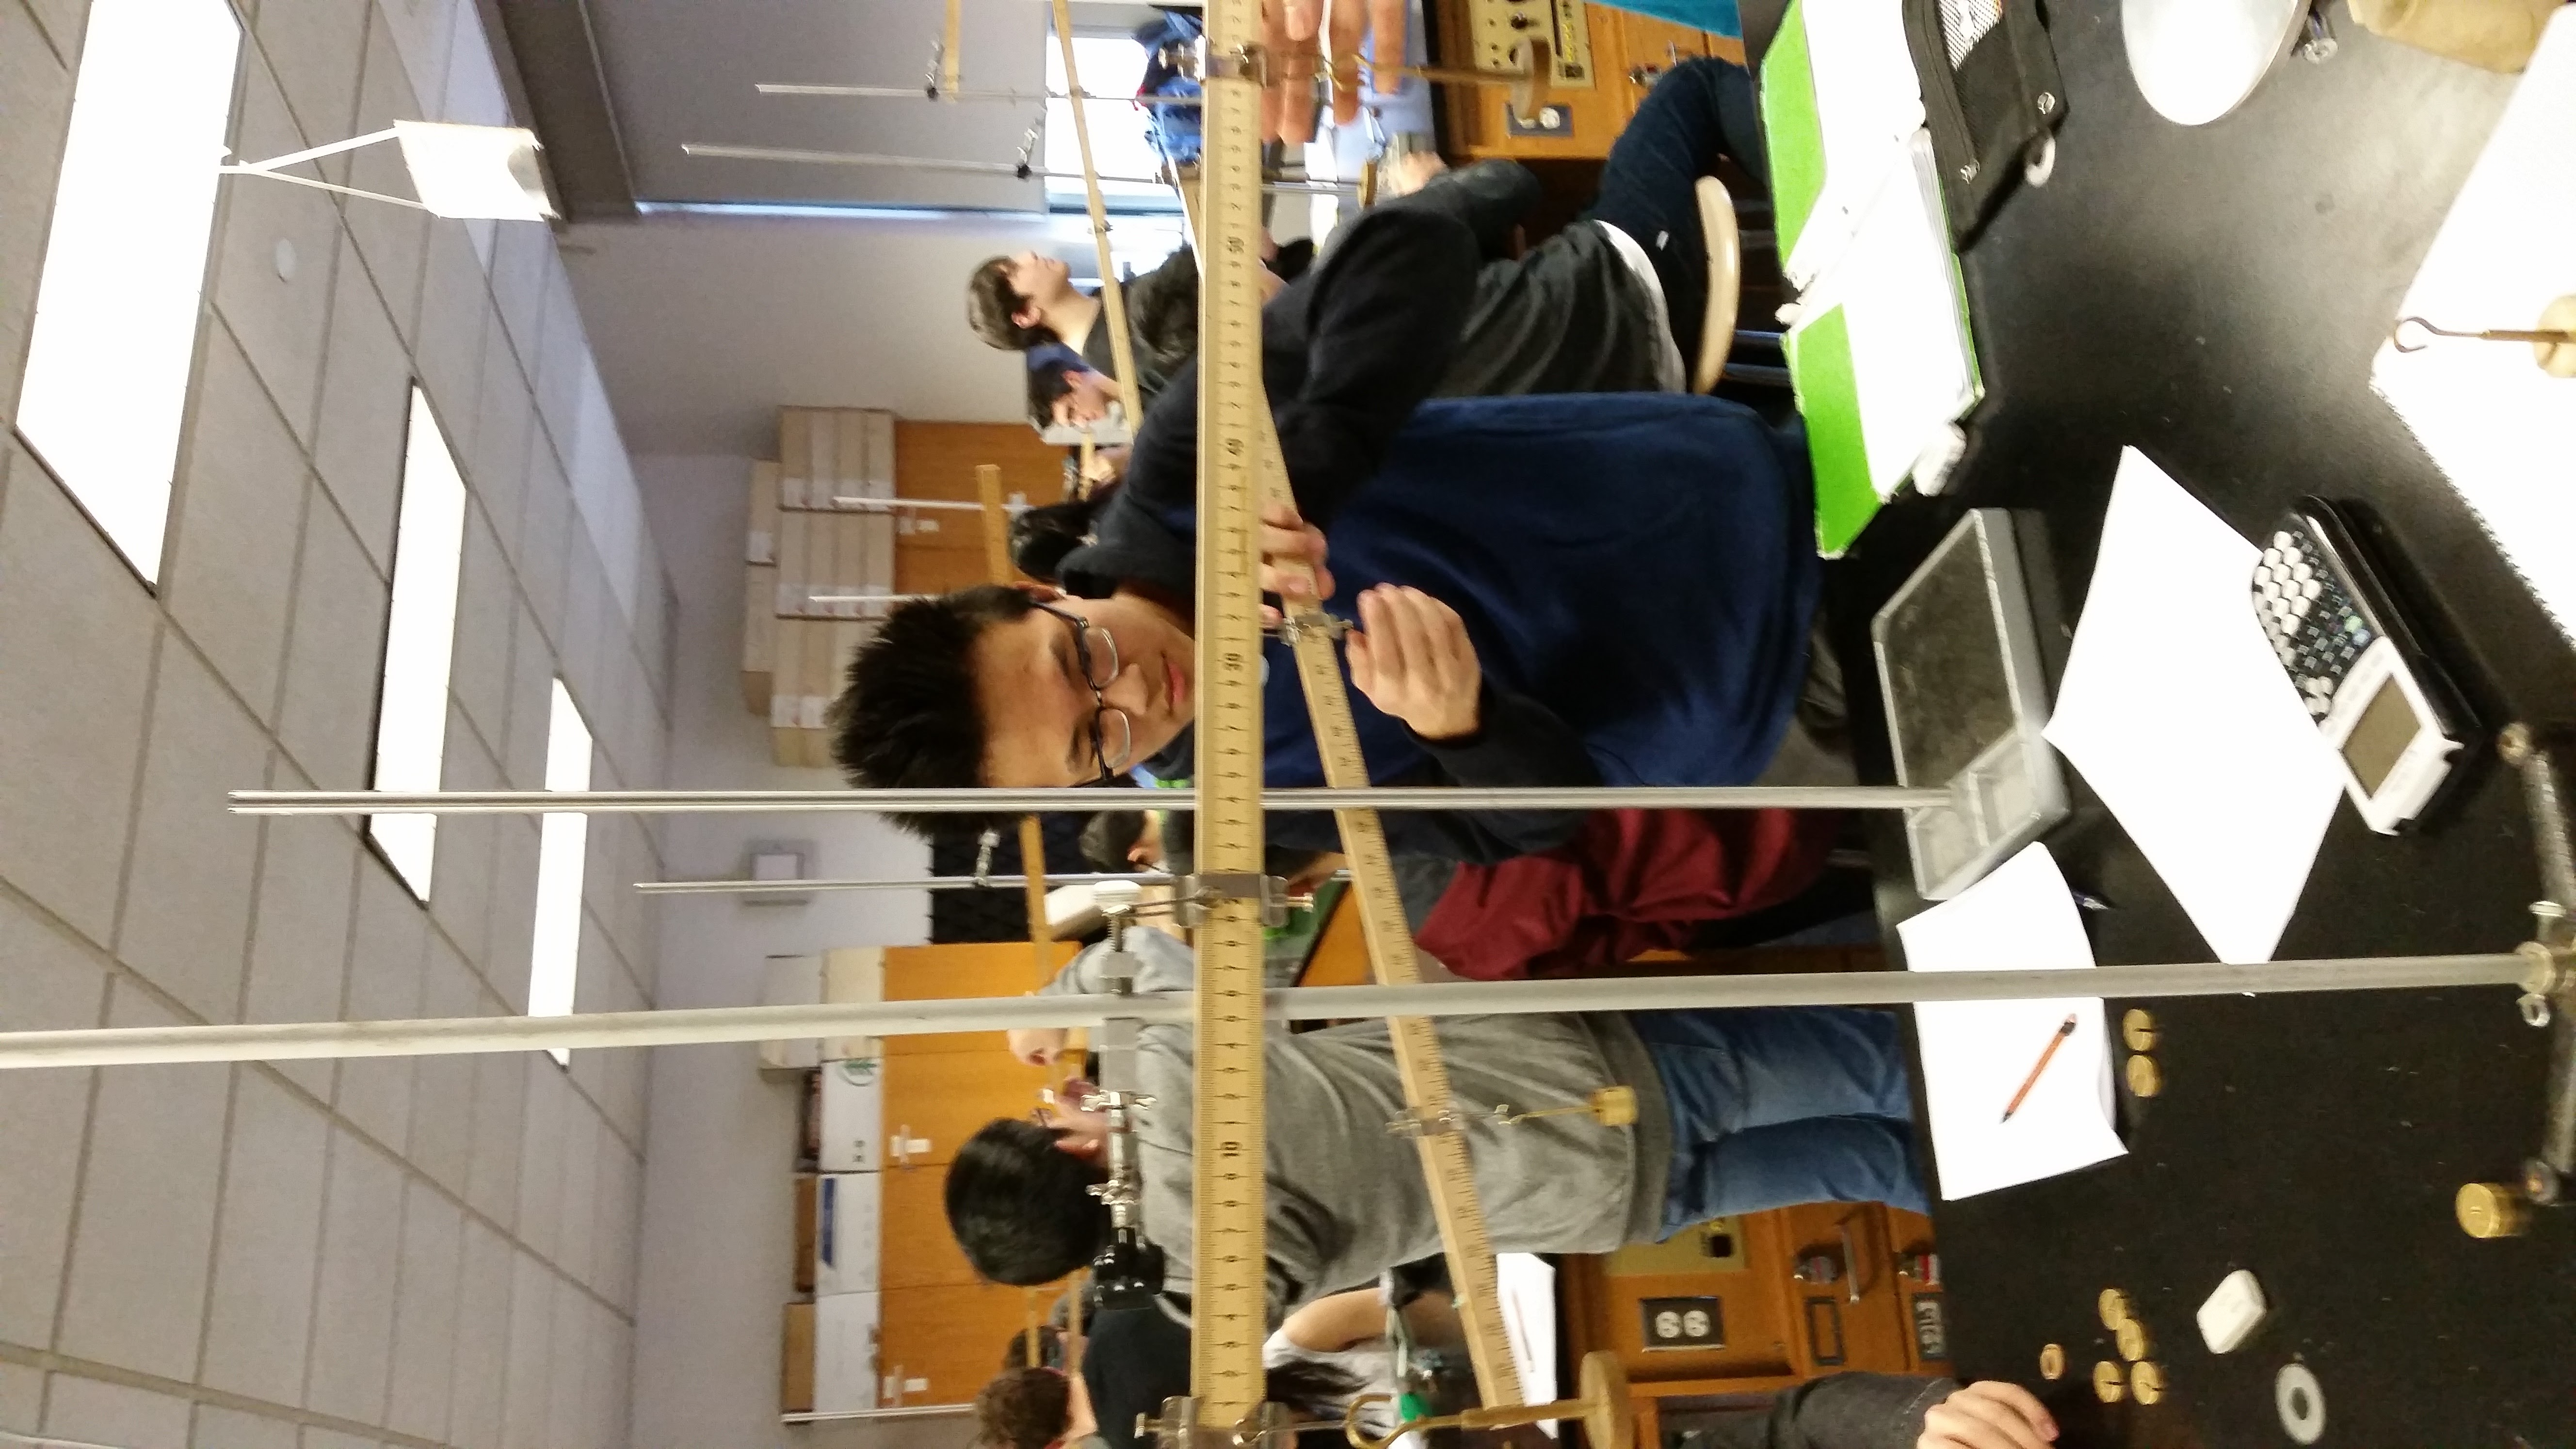
\includegraphics[scale=0.15, angle=270]{lab4.jpg}
\vspace*{19cm}
\end{figure}

\begin{center}
$$\text{Center of Gravity} (x_0) = 0.5 m$$
$$m_m \text{(Mass of Meterstick)} = 0.0631 kg$$
$$m_c \text{(Mass of a Clamp)} = 0.01663 kg$$
\begin{tabular}
{|m{7em}|m{14em}|m{14em}|}
\hline
Case Number & Masses (kg) & Coordinate (m)\\
\hline
Case 1 & $m_1 = 0.1, m_2 = 0.2$ & $x_1 = 0.15, x_2 = 0.677$ \\
\hline
Case 2a & $m_1 = 0.1, m_2 = 0.2, m_3 = 0.05$ & $x_1 = 0.3, x_2 = 0.7, x_3 = 0.031$ \\
\hline
Case 2b & $m_1 = 0.1, m_2 = 0.2, m_3 = 0.05$ & $x_1 = 0.2, x_2 = 0.6, x_3 = 0.693$ \\
\hline
Case 3 & $m_1 = 0.17, m_2 = 0.2$ & $x_1 = 0.1, x_2 = 0.845$ \\
\hline
Case 5 & $m_1 = 0.1$ & $x_1 = 0, x_o' \text{(support point)} = 0.201$ \\
\hline
Case 6a & $m_1 = 0.1, m_2 = 0.1$ & $x_1 = 0, x_2 = 0.6, x_o' = 0.351$\\
\hline
Case 6b& $m_1 = 0.1, m_2 = 0.1$ & $x_1 = 0, x_2 = 0.7, x_o' = 0.388$\\
\hline
Case 6c& $m_1 = 0.1, m_2 = 0.1$ & $x_1 = 0, x_2 = 0.8, x_o' = 0.425$\\
\hline
Case 6d& $m_1 = 0.1, m_2 = 0.1$ & $x_1 = 0, x_2 = 0.9, x_o' = 0.462$ \\
\hline
\end{tabular}
\end{center}

\section*{Discussion}
Sample calculations for the non-measured data are as shown:

$$\mu = \frac{m_{s}}{L} = \frac{0.0631}{1} = 0.0631 kg/m$$
$$\text{Moment/Lever Arm (Case 1)} (r_1) = |x_o - x_1| = |0.5 - 0.15| = 0.35$$
$$\tau_{1} \text{(Case 1)} = r_1F_1 = r_1(m_1 + m_c)g = 0.35*(0.1 + 0.01663)*9.8 = 0.4 N*m$$
$$\tau_{cc} \text{(Case 2a)} = \sum_{n}\tau^{\text{left}}_n = \tau_1 + \tau_3 = 0.535 N*m$$
$$\text{Percent Difference (Case 1)} = \frac{|\tau_{cc} - \tau_{cw}|}{\tau{cc}} * 100\%  = \frac{|0.4 - 0.376|}{0.4} * 100\% = 6\%$$
$$\text{Percent Error (Case 2b)} = \frac{|r_{3calc} - r_{3meas}|}{r_{3calc}} * 100\% = \frac{|0.693 - 0.659|}{0.659} * 100\% = 5.16\%$$

Other calculations:
$$r_3 \text{(Case 2b, Calulated)} = \frac{\tau_{cc} - \tau_2}{g*(m_3+m_c)} = \frac{0.3429 - 9.8*0.2*0.1}{9.8*0.05} = 0.225 m$$
$$m_1 \text{(Case 3, Calculated)} = \frac{\tau_{cw}}{g*r_1} = \frac{0.7324}{9.8*0.4} = 0.187 kg$$
$$r_2 \text{(Case 5a)} = |x_0' - x_2| = |x_0' - (x_0' + \frac{L - x_0'}{2})| = \frac{L - x_0'}{2} = \frac{1 - 0.201}{2} = 0.3995 m$$
$$m_2 \text{(Case 5a)} = m_{s} = 0.0631 kg$$
$$m_2 \text{(Case 5b)} = \mu*l = \mu*(L - x_o') = 0.0631*(1 - 0.201) = 0.0504 kg$$

\begin{center}
\begin{tabular}
{|m{7em}|m{7em}|m{7em}|m{7em}|m{7em}|}
\hline
Case Number & Moment/Lever Arms (m) & Counterclockwise Torque (N*m) & Clockwise Torque (N*m) & Percent Error (Value)\\
\hline
Case 1 & $r_1 = 0.35, r_2 = 0.177$ & 0.4 & 0.376 & 6 (Torque)\\
\hline
Case 2a & $r_1 = 0.2, r_2 = 0.2, r_3 = 0.469$ & 0.535 & 0.425 & 25.8 (Torque)\\
\hline
Case 2b & $r_1 = 0.3, r_2 = 0.1, r_3 = 0.193$ & 0.3429 & 0.3383 & 14.2 ($r_3$)\\ 
\hline
Case 3 & $r_1 = 0.4, r_2 = 0.345$ & 0.7316 & 0.7324 & 9.09 ($m_1$)\\
\hline
Case 5a & $r_1 = 0.201, r_2 = 0.3995$ & 0.2297 & 0.247 & 7.004 (Torque) \\
\hline
Case 5b & $r_1 = 0.201, r_2 = 0.3995, r_3 = 0.1005$ & 0.2422 & 0.1973 & 18.54 (Torque) \\
\hline
Case 6a & $r_1 = 0.351, r_2 = 0.249$ & - & - & - \\ 
\hline
Case 6b & $r_1 = 0.388, r_2 = 0.312$ & - & - & - \\
\hline
Case 6c & $r_1 = 0.425, r_2 = 0.375$ & - & - & - \\
\hline
Case 6d & $r_1 = 0.462, r_2 = 0.438$ & 0.594 & 0.59 & 0.673 (Torque) \\
\hline
\end{tabular}
\end{center}

Part 5 Torque Difference Percent Difference:
$$\tau_{5a-diff} = |\tau_{5a-cc} - \tau_{5a-cw}| = |0.2297 - 0.247| = 0.0173 N*m$$
$$\tau_{5b-diff} = 0.0449 N*m$$
$$\text{Percent Difference} = 61.47\%$$

Part 6 Predictions:
$$\text{Part 6 Prediction} (x_o') = 0.462 m$$
$$\text{Percent Difference} = 0\%$$

\begin{figure}[p]
\centering
\hspace*{-12cm}
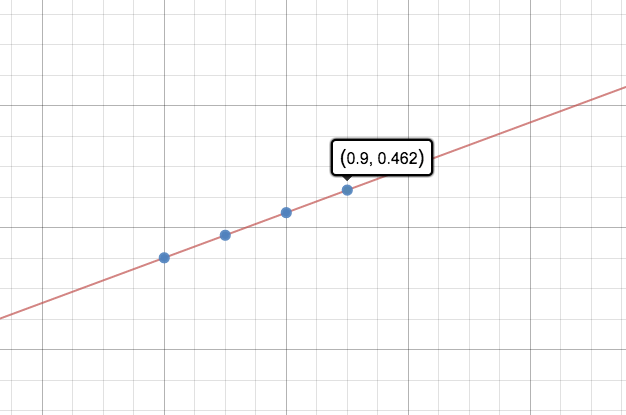
\includegraphics[scale=0.9, angle=0]{graph4.jpg}
\vspace*{0cm}
\end{figure}

Force is considered to be at equilibrium, due to the meterstick being clamped to the support, such that while it is able to rotate, the clamp provides the normal force to balance out the overall weight of the apparatus.

One possible cause of error for Case 3 specifically, was the imprecise nature of the masses, such that the value found was an approximation using the sizes provided. In addition, Case 5a was likely to have error, due to assuming the entire mass of the yardstick was concentrated on the right of the balance point. We also assumed that the linear density of the yardstick was constant, which is theoretically true, but realistically could cause an error in the data. Finally, since the masses are not point masses, that could introduce error, such that they don't exert the exact intended torque on the meterstick. Otherwise, most of our percent errors were below 20\%, many below 10\%, especially the results of Case 6, showing the validity of the model itself. 

\section*{Conclusion}
Case 1 had an experimental torque of 0.376 N*m to the real torque of 0.4 N*m for a percent error of 6\%. Case 2a had an experimental torque of 0.535 N*m to the real torque of 0.425 N*m for a percent error of 25.8\%. Case 2b had a real torque of 0.3429 N*m and an experimental torque of 0.3383 N*m, such that the experimental moment arm 3, $r_3$, was 0.193 m to the real 0.225 m, for a percent error of 14.2\%. Case 3 had an experimental torque of 0.7316 N*m to the real torque of 0.7324 N*m, such that the experimental mass, $m_1$, was 0.17 kg to the real mass, 0.187 kg, for a percent error of 9.09\%.

Case 5a had a counterclockwise torque approximation of 0.2297 N*m, and a clockwise torque approximation of 0.247 N*m for a 7.004\% difference. Case 5b has a 0.2422 N*m counterclockwise torque approximation, and a 0.1973 N*m clockwise torque approximation for a 18.54\% difference.

Case 6d found $x_o'$ experimentally of 0.462 m, the exact predicted point based on the linear approximation of the previous data points, such that the real torque of 0.594 N*m was experimentally found as 0.59 N*m, for a percent error of torque of 0.673\% and a percent difference of $x_o'$ of 0\%.

\end{document}
